\pdfsuppresswarningpagegroup=1

\documentclass{beamer}
\usetheme{Boadilla}
\usecolortheme{seahorse}
\usepackage{pifont}
\usepackage{svg}
\usepackage{t1enc}
\usepackage[hungarian]{babel}

\titlegraphic{
\includegraphics[width=2cm]{elte_cimer_szines}}
\title[HoloDB]{HoloDB: szintetikus adatok on-the-fly szolgáltatása relációs adatbázisként}
\author[Horváth Dávid]{Horváth Dávid \\ ~ \\ { \footnotesize Témavezető: Dr. Vincellér Zoltán, Mesteroktató }}
\institute[ELTE-IK]{ELTE Informatikai Kar, Információs Rendszerek Tanszék}
\date{2023}

\newcommand{\condpause}{\pause}
%\newcommand{\condpause}{}

\newcommand{\slidetitle}[2]{\frametitle{{\small #1 ~ \ding{226} ~ } \normalsize #2}}

\begin{document}
\beamertemplatenavigationsymbolsempty

\frame{\titlepage}

\AtBeginSection[]
{
    \begin{frame}
        \frametitle{Tartalom}
        \tableofcontents[currentsection]
    \end{frame}
}

\section{Bevezetés: adatbázist akarok, most!}
\def\sectionshorttitle{Bevezetés}

\begin{frame}
    \slidetitle{\sectionshorttitle}{TODO}
    TODO
\end{frame}

\section{Körkép: a létező (kerülő)megoldások}
\def\sectionshorttitle{Körkép}

\begin{frame}
    \slidetitle{\sectionshorttitle}{TODO}
    TODO
\end{frame}

\section{Egy új megoldás körvonalai: HoloDB}
\def\sectionshorttitle{HoloDB}

\begin{frame}
    \slidetitle{\sectionshorttitle}{TODO}
    TODO
\end{frame}

\section{A HoloDB architektúrája}
\def\sectionshorttitle{Architektúra}

\begin{frame}
    \slidetitle{\sectionshorttitle}{TODO}
    TODO
\end{frame}

\section{A szűk keresztmetszet: értékkiosztások}
\def\sectionshorttitle{Értékkiosztások}

\begin{frame}
    \slidetitle{\sectionshorttitle}{XXXXXXXXXXXX}

    Mik ezek? Mit kell megoldjanak?
\end{frame}

\begin{frame}
    \slidetitle{\sectionshorttitle}{Általános kétfázisú értékkiosztás}
    
    \centering
    
    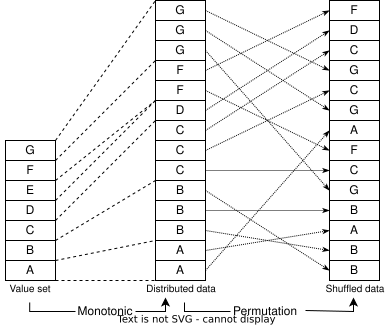
\includegraphics[height=0.5\textwidth]{diagram/distribution}
    
    Kétfázisú értékkiosztás alapelve: \par
    visszafejthető disztribúció és permutáció kompozíciója
\end{frame}

\begin{frame}
    \slidetitle{\sectionshorttitle}{Kétfázisú értékkiosztás: adatlekérés}
    
    \centering
    
    \includegraphics[height=0.45\textwidth]{diagram/getvalue-0}
    
    \hspace{0.7cm}
    
    Adatlekérés a kétfázisú értékkiosztásból
\end{frame}

\begin{frame}[noframenumbering]
    \slidetitle{\sectionshorttitle}{Kétfázisú értékkiosztás: adatlekérés}
    
    \centering
    
    \includegraphics[height=0.45\textwidth]{diagram/getvalue-1}
    
    \hspace{0.7cm}
    
    Adatlekérés a kétfázisú értékkiosztásból
\end{frame}

\begin{frame}[noframenumbering]
    \slidetitle{\sectionshorttitle}{Kétfázisú értékkiosztás: adatlekérés}
    
    \centering
    
    \includegraphics[height=0.45\textwidth]{diagram/getvalue-2}
    
    \hspace{0.7cm}
    
    Adatlekérés a kétfázisú értékkiosztásból
\end{frame}

\begin{frame}[noframenumbering]
    \slidetitle{\sectionshorttitle}{Kétfázisú értékkiosztás: adatlekérés}
    
    \centering
    
    \includegraphics[height=0.45\textwidth]{diagram/getvalue-3}
    
    \hspace{0.7cm}
    
    Adatlekérés a kétfázisú értékkiosztásból
\end{frame}

\begin{frame}[noframenumbering]
    \slidetitle{\sectionshorttitle}{Kétfázisú értékkiosztás: adatlekérés}
    
    \centering
    
    \includegraphics[height=0.45\textwidth]{diagram/getvalue-4}
    
    \hspace{0.7cm}
    
    Adatlekérés a kétfázisú értékkiosztásból
\end{frame}

\begin{frame}
    \slidetitle{\sectionshorttitle}{Kétfázisú értékkiosztás: keresés}
    
    \centering
    
    \includegraphics[height=0.45\textwidth]{diagram/findvalue-0}
    
    \vspace{0.5cm}
    
    Keresés a kétfázisú értékkiosztásban: \par
    A megfordíthatóság biztosítja a hatékony keresést
\end{frame}

\begin{frame}[noframenumbering]
    \slidetitle{\sectionshorttitle}{Kétfázisú értékkiosztás: keresés}
    
    \centering
    
    \includegraphics[height=0.45\textwidth]{diagram/findvalue-1}
    
    \vspace{0.5cm}
    
    Keresés a kétfázisú értékkiosztásban: \par
    A megfordíthatóság biztosítja a hatékony keresést
\end{frame}

\begin{frame}[noframenumbering]
    \slidetitle{\sectionshorttitle}{Kétfázisú értékkiosztás: keresés}
    
    \centering
    
    \includegraphics[height=0.45\textwidth]{diagram/findvalue-2}
    
    \vspace{0.5cm}
    
    Keresés a kétfázisú értékkiosztásban: \par
    A megfordíthatóság biztosítja a hatékony keresést
\end{frame}

\begin{frame}[noframenumbering]
    \slidetitle{\sectionshorttitle}{Kétfázisú értékkiosztás: keresés}
    
    \centering
    
    \includegraphics[height=0.45\textwidth]{diagram/findvalue-3}
    
    \vspace{0.5cm}
    
    Keresés a kétfázisú értékkiosztásban: \par
    A megfordíthatóság biztosítja a hatékony keresést
\end{frame}

\begin{frame}
    \slidetitle{\sectionshorttitle}{Az értékkészlet interfész-tulajdonságai}
    
    \begin{itemize}
        \setlength\itemsep{1em}
        \item Rendezett \condpause
        \item Nincs ismétlődés (unique) \condpause
        \item Lekérhető a lista hossza \condpause
        \item Lekérhető az adott pozíción lévő érték (random access) \condpause
        \item Lekérhető az adott érték pozíciója (reverse index) \condpause \par
              ~ ~ ~ (ha az érték nem található, akkor a rendezés szerinti helye) \condpause
        \item A lekérések gyorsan hajtódnak végre
    \end{itemize}
\end{frame}

\begin{frame}
    \slidetitle{\sectionshorttitle}{Tipikus értékkészletek}
    
    \begin{itemize}
        \setlength\itemsep{1em}
        \item Szavak/kifejezések előre adott, rendezett listája \condpause
        \item Numerikus sáv (például számok 1-től $n$-ig) \condpause
        \item Reguláris kifejezésre illeszkedő szövegek \condpause
        \item 
    \end{itemize}
\end{frame}

\section{Eredmények}
\def\sectionshorttitle{Eredmények}

\begin{frame}
    \slidetitle{\sectionshorttitle}{TODO}
    TODO
\end{frame}

\section{Összegzés}
\def\sectionshorttitle{Összegzés}

\begin{frame}
    \slidetitle{\sectionshorttitle}{TODO}
    TODO
\end{frame}

\end{document}
